\chapter{Configuring the TransistorTester}
\label{sec:config}
The complete software for the TransistorTester is available in source code.
The compilation of modules is controlled with a Makefile. The developement was done
at the Ubuntu Linux operating system with the GNU toolchain (gcc version 4.5.3).
It should be possible to use other Linux operating systems without problems.
To load the compiled data to the flash memory or
the EEprom memory, the tool avrdude (version 5.11svn) was taken by the Makefile, if you call ``make upload''.
 The program avrdude \cite{avrdude} is available for Linux and Windows operating system.
The gnu C-compiler gcc is also taken by the AVR studio software and
by the WinAVR \cite{winavr1},\cite{winavr2} software at the Windows operating system.
You can load the program data (.hex and .eep) also with other tools to the ATmega,
but only my Makefile version takes care to load the correct data to the choosed processor.
Avrdude loads only data to the ATmega if the Signature Bytes of the connected ATmega is
identical to the choosed one. 
If you alter the Makefile, all the software will be compiled new, if you call a ``make'' or
``make upload'' command. The software compiled for a ATmega8 does not run on a ATmega168.
The software compiled for a ATmega328 does not run on the ATmega168! 
A exeption fron this rule is the software compiled for ATmega168, this data can also be used
for a ATmega328 without changes.
Be careful, if you don't use my Makefile.

With the correct options set, my software runs on the unchanged hardware of Markus F.
(PARTNO=M8, NO option NO\_AREF\_CAP and NO PULLUP\_DISABLE option).
The clock rate can also be set to 8 MHz with fuses, no crystal is required!


The following options in the Makefile are avaiable to configure the software for your Tester.

\begin{description}
  \item[PARTNO] describes the target processor:\\
         m8 = ATmega8\\
         m168 or m168p = ATmega168\\
         m328 or m328p = ATmega328\\
    example:  PARTNO = m168
  \item[UI\_LANGUAGE] specifies the favored Language\\
    LANG\_ENGLISH, LANG\_GERMAN, LANG\_POLISH, LANG\_CZECH, LANG\_SLOVAK, LANG\_SLOVENE, LANG\_DUTCH, LANG\_BRASIL,
 LANG\_RUSSIAN and LANG\_UKRAINIAN is currently avaiable.
 The russian or ukrainian language requires a LCD with cyrillic character set.\\
    example:  UI\_LANGUAGE = LANG\_ENGLISH
  \item[LCD\_CYRILLIC] is only needed for a LCD-display with cyrillic character set. The \(\mu\) and \(\Omega\) character
is not avaiable with the cyrillic character set.
If you specify this option, both characters are loaded to the LCD with software.\\
example: CFLAGS += -DLCD\_CYRILLIC
 \item[LCD\_DOGM] must be set, if a LCD with ST7036 controller (Type DOG-M) is used for displaying.
The LCD-contrast is then set with software commands.\\
example: CFLAGS += -DLCD\_DOGM
  \item[STRIP\_GRID\_BOARD] This option adapts the software to a changed port D connection for strip grid printed boards.
You can find the details in the chapter hardware \ref{sec:hardware}.
  \item[WITH\_SELFTEST] If you specify this Option, software will include a selftest function.
Selftest will be started, if you connect all three probes together and start measurement.\\
example: CFLAGS += -DWITH\_SELFTEST
  \item[AUTO\_CAL] The zero offset for capacity measurement will be written additionally
to the EEprom with the selftest routine. Additionally the offset voltage of the analog comparator (REF\_C\_KORR) and the
voltage offset of the internal reference voltage (REF\_R\_KORR) will be measured automatically, if you connect a
capacitor with a capacity value between \(100 nF\) and \(20 \mu F\) to pin~1 and pin~3 after measurement of capacity zero offset. 
All found values will be written to EEprom and will be used for further measurements automatically.
The port output resistance values will be determined at the beginning of each measurement.\\
example: CFLAGS += -DAUTO\_CAL
  \item[FREQUENCY\_50HZ] At the end of selftest a 50~Hz Signal will be generated on Port~2 and Port~3 for up to one minute.\\
example: CFLAGS += -DFREQUENCY\_50HZ
  \item[CAP\_EMPTY\_LEVEL]  This option defines the voltage level for discharged capacitor (mV units).
You can set the level to higher value as 3mV, if the tester does not finish discharging of capacitors.
In this case the tester ends after longer time with the message ``Cell!''.\\
example: CFLAGS += -DCAP\_EMPTY\_LEVEL=3
  \item[WITH\_AUTO\_REF] specifies, that reference voltage is read to get the actual factor for capacity measuring of low capacity values (below \(40\mu F\)).\\
example:  CFLAGS += -DWITH\_AUTO\_REF
  \item[REF\_C\_KORR] specifies a offset for readed reference voltage in mV units.
This can be used to adjust the capacity measurement of little capacitors.
A correction value of 10 results to about 1~percent lower measurement results.
If the option AUTO\_CAL is selected together with the WITH\_SELFTEST option, the REF\_C\_KORR will be
a offset to the measured voltage difference of the test capacitor and the internal reference voltage.\\
example:  CFLAGS += -DREF\_C\_KORR=14
  \item[REF\_L\_KORR] specifies a additional offset in mV units to the reference voltage for the measurement of
inductance values. 
The REF\_C\_KORR offset and respectively the offset value from the calibration is additionally used with the inductance measurement.
The REF\_L\_KORR value will be subtracted for measurements without a \(680 \Omega\) resistor,
for measurements with a \(680 \Omega\) resistor the value will be added.\\
example: CFLAGS += -DREF\_L\_KORR=40
  \item[C\_H\_KORR] specifies a correction value for the measurement of big capacitor values.
A value of 10 results to 1~percent lower measurement results.\\
example:  CFLAGS += -DC\_H\_KORR=10
  \item[WITH\_UART] uses the pin PC3 as output for the serial text (V24).
If the option is not set, the pin PC3 can be used for reading a external voltage with a 10:1 resistor divider.
With this equipment you can check the breakdown voltage of zener diodes, which have more than 4.5V breakdown voltage.
This measurement will repeat with 3 measurements per second until you release the Start button.\\
example: CFLAGS += -DWITH\_UART
  \item[AUTOSCALE\_ADC] enables the automatic scale switchover of the ADC to either VCC or internal reference.
Internal reference gives a 2.56V scale for ATmega8 and a 1.1V scale for other processors.\\
example: CFLAGS += -DAUTOSCALE\_ADC
  \item[ESR\_ZERO] defines a zero offset for ESR measurements.
The zero offsets for all three pin combinations will be determined with the selftest and replaces the preset zero offset.
This zero offsets will be subtracted from all ESR measurements.
Example: CFLAGS += -DESR\_ZERO=29
  \item[NO\_AREF\_CAP] tells your Software, that you have no capacitor (\(100 nF\)) installed at pin AREF (pin 21).
This enables a shorter wait-time for the AUTOSCALE\_ADC scale switching of the ADC.
A \(1 nF\) capacitor was tested in this mode without detected errors.
Figure \ref{pic:aref1} and \ref{pic:aref5} show the switching time with a \(1 nF\) capacitor.
As you can see the switching from 5V to 1.1V is much slower than switching back to 5V. If you
have still installed the \(100 nF\), switching time will be about factor 100 longer!\\
example: CFLAGS += -DNO\_AREF\_CAP
  \item[REF\_R\_KORR] specifies a offset for the internal ADC-reference voltage in mV units.
With this offset a difference by switching from VCC based ADC reference to internal ADC reference for resistor measurement can be adjusted.
If you select the AUTO\_CAL option of the selftest section, this value is only a additionally offset to the found voltage 
difference in the AUTO\_CAL function.\\
example: CFLAGS += -DREF\_R\_KORR=10
  \item[OP\_MHZ] tells your software at which Clock Frequency in MHz your Tester will operate.
The software is tested only for 1 MHz, 8MHz and additionally 16MHz. 
The 8MHz operation is recommended for better resolution of capacity and inductance measurement.\\
example: OP\_MHZ = 8
  \item[RESTART\_DELAY\_TICS] must be set to 6, if the ATmega168 or ATmega328 is used with the internal RC-oszillator instead of
the crystal oszillator.
If this value is not preset, the software respects the 16384 clock tics delay for restart from sleep mode with the crystal operation.\\
example: CFLAGS += -DRESTART\_DELAY\_TICS=6
  \item[USE\_EEPROM] specifies if you wish to locate fix text and tables in EEprom Memory. Otherwise the flash memory is used.
Recommended is to use the EEprom (option set).\\
example: CFLAGS += -DUSE\_EEPROM
\item[EBC\_STYLE] specifies, that the output of transistor pin layout is done with format ``EBC=...'' or ``GDS=...''.
This way of output save program memory for the ATmega. Without this option the layout is shown with the
format ``123=...'', where every point represent a E~(Emitter), B~(Base) or C~(Collector).
For FET transistors every point can be a G~(Gate), D~(Drain) or S~(Source).
If the sequence of the test pins is not 1, 2 and 3 in the reading direction, you can invert the sequence with the option
EBC\_STYLE=321 . The pin assignment is then shown with style ''321=...'', which will better match the usual
reading direction.\\
Example: CFLAGS += EBC\_STYLE
  \item[NO\_NANO] specifies that the decimal prefix nano will not be used to display the measurement results.
So capacity values will be shown in \(\mu F\) instead of \(nF\).\\
Example: CFLAGS += NO\_NANO
\item[PULLUP\_DISABLE] specifies, that you don't need the internal pull-up resistors.
 You must have installed a external pull-up resistor at pin~13 (PD7) to VCC, if you use this option.
This option prevents a possible influence of pull-up resistors at the measuring ports (Port~B and Port~C).\\
example: CFLAGS += -DPULLUP\_DISABLE
  \item[ANZ\_MESS] this option specifies, how often an ADC value is read and accumulated.
You can select any value between 5 and 200 for building mean value of one ADC measurement.
Higher values result to better accuracy, but  longer measurement time.
One ADC measurement with 44~values takes about 5ms.\\
example: CFLAGS += -DANZ\_MESS=25
  \item[POWER\_OFF] This option enables the automatic power off function. If you don't specify this option,
 measurements are done in a loop infinitely  until power is disconnected with a ON/OFF switch.
If you have the tester without the power off transistors, you can deselect the option POWER\_OFF.

If you have NOT selected the POWER\_OFF option with the transistors installed,
you can also shut down the tester.
During displaying the measurement result you should hold the start key pressed for several seconds until
the ''Timeout'' message is displayed.  If you then release the key, the tester will be shut off.

You can also specify, after how many measurements without a founded part the tester will shut down.
The tester will also shut down the power after twice as much measurements are done in sequence without a
single failed part search. If you have forgotten to unconnect a test part, total discharging of battery is avoided. 
Specify the option with a form like CFLAGS += -DPOWER\_OFF=5 for a shut off after 5 consecutive measurements
without part found. Also 10~measurements with any founded part one after another will shut down.
Only if any sequence is interrupted by the other type, measurement continues.
The result of measurement stay on the display for 14~seconds for the single measurement, for the
multiple measurement version display time is reduced to 5~seconds (set in config.h).
If the start key is pressed a longer time on power on time, the display time is also 14~seconds for the multiple measurement.
The maximum value is 255 (CFLAGS += -DPOWER\_OFF=255).\\
example 1: CFLAGS += -DPOWER\_OFF=5\\
example 2: CFLAGS += -DPOWER\_OFF
  \item[BAT\_CHECK] enables the Battery Voltage Check. If you don't select this option, the version number of
software is output to the LCD instead.
This option is usefull for battery powered tester version to remember for the battery change.\\
example: CFLAGS += -DBAT\_CHECK
  \item[BAT\_OUT] enables Battery Voltage Output on LCD (if BAT\_CHECK is selected).
 If your 9V supply has a diode installed, use the BAT\_OUT=600 form to specify the threshold voltage (mV) of your diode
to adjust the output value.
Also the voltage loss of transistor T3 can be respected with this option.
 threshold level does not affect the voltage checking levels (BAT\_POOR).\\
example 1: CFLAGS += -DBAT\_OUT=300\\
example 2: CFLAGS += -DBAT\_OUT
  \item[BAT\_POOR] sets the poor level of battery voltage to the specified 1mV value.
The warning level of battery voltage is 0.8V higher than the specified poor level, if the poor level is more than 5.3V.
If the poor level is 5.3V or less, the warning level is 0.4V higher. If the poor level is below 3.25V, the
warning level is only 0.2V higher than the selected poor level and if the poor level is below 1.3V, the
warning level is only 0.1V higher than the specified poor level.
Setting the poor level to low values such as 5.4V is not recommended for rechargeable 9V batteries,
because this increase the risk of battery damage by the reason of the deep discharge!
If you use a rechargeable 9V Battery, it is recommended to use a Ready To Use type, because of the lower self-discharge.\\
example for low drop regulator (5.4V): CFLAGS += -DBAT\_POOR=5400\\
example for 7805 type regulator (6.4V): CFLAGS += -DBAT\_POOR=6400
  \item[INHIBIT\_SLEEP\_MODE] disable the use of the sleep mode of the processor.
Normaly the software uses for longer work breaks the sleep mode to avoid unneeded current consumption.
The usage of this sleep mode indeed spare battery capacity, but produce additional stress for the voltage regulator.\\
example: CFLAGS += -DINHIBIT\_SLEEP\_MODE

  \item[PROGRAMMER] select your programmer type for avrdude interface program.
The correct selection of this option is needed, if you use the ``make upload'' or ``make fuses'' call
of this Makefile.
For further information please look to the manual pages of avrdude and online documentation~\cite{avrdude}.\\
example: PROGRAMMER=avrisp2
  \item[BitClock] selects the Bit clock period for the Programmer. See the description of the -B parameter of avrdude.\\
example: BitClock=5.0
  \item[PORT] select the port where avrdude can reach your microcontroller (atmega).
For further information please look to the manual pages of avrdude.\\
example: PORT=usb

\end{description}

\begin{figure}[H]
  \begin{subfigure}[b]{9cm}
    \centering
    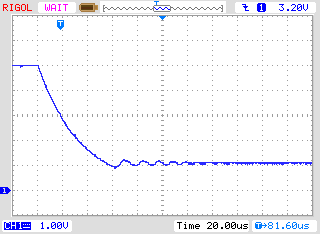
\includegraphics[width=9cm]{../PNG/AREF2_1V.png}
    \caption{from 5V to 1.1V }
    \label{pic:aref1}
  \end{subfigure}
  ~
  \begin{subfigure}[b]{9cm}
    \centering
    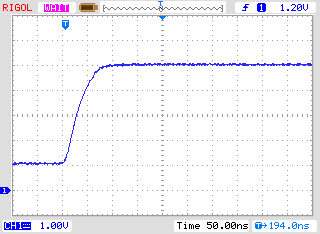
\includegraphics[width=9cm]{../PNG/AREF2VCC.png}
    \caption{from 1.1V to 5V}
    \label{pic:aref5}
  \end{subfigure}
  \caption{AREF switching with a \(1nF\) Capacitor}
\end{figure}


Additional parameters can be set in the files transistortester.h and config.h .
The file transistortester.h contains global variables and defines the port / pin constellation
and the resistor values used for measurement.
The file config.h specifies parameter for different processor types, wait times and the clock
frequency of the ADC. Normally there is no reason to change these values.
